\chapter{Alarm}
\section{Inleiding}
In de alarm module wordt een led aangestuurd, die 15 minuten voor de ingestelde tijd in de main controller begint met branden en steeds feller wordt naarmate de tijd verstrijkt. Als de huidige tijd gelijk is aan de ingestelde tijd brandt de led op z'n felst en gaat er een geluid af, totdat er een knop wordt ingedrukt.

\section{Specificaties}
\subsection{Ingangen}
\begin{itemize}[nolistsep]
\item Klok, standaard input.
\item Reset, standaard input.
\item Tijd-uur, huidige tijd in uren.
\item Tijd-minuut, huidige tijd in minuten.
\item Wekker-uur, uur ingesteld in de main controller.
\item Wekker-min, minuten ingestels in de main controller.
\item Sec, seconde signaal gegenereerd in de DCF controller.
\item Knop, alarm uitschakelen.
\end{itemize}

\subsection{Uitgangen}
\begin{itemize}[nolistsep]
\item PWM-signaal, signaal om de led aan te sturen.
\item Geluid, signaal om een geluid af te laten gaan.
\end{itemize}

\subsection{Gedrag}
Het alarm moet een bepaalde tijd voordat de wekker is ingesteld aangaan, nu gekozen voor 15 minuten.
Er wordt 15 minuten van de ingestelde tijd afgetrokken. Zodra die tijd gelijk is aan de huidige tijd komt er een signaal (licht) aan bij het gedeelte wat voor een pwm signaal zorgt.
In dat gedeelte wordt een pwm signaal gegenereerd dat elke 15 seconde breder wordt. Dit wordt gedaan door in een counter 15 seconde te tellen. Elke 15 seconde wordt de variable "lenght" kleiner. Deze begon op 64 en wordt vergeleken met een andere counter die elke klokflank telt, tot 64. Als de counter groter of gelijk is aan "length" dan is het pwm-signaal hoog. 
Als 15 minuten zijn verstreken na het aangaan van de led, dus de ingestelde tijd is gelijk aan de huidige tijd, brandt de led op z'n felst. Ook zal dan een "geluid" signaal naar '1' gaan. Dit blijft zo totdat de knop wordt ingedrukt of alles wordt gereset.
\newpage
\section{Functionaliteit}
\subsection{FSM}
FSM van ``alarm-compare", het gedeelte waar de tijd vergeleken wordt met de ingestelde wekker tijd.

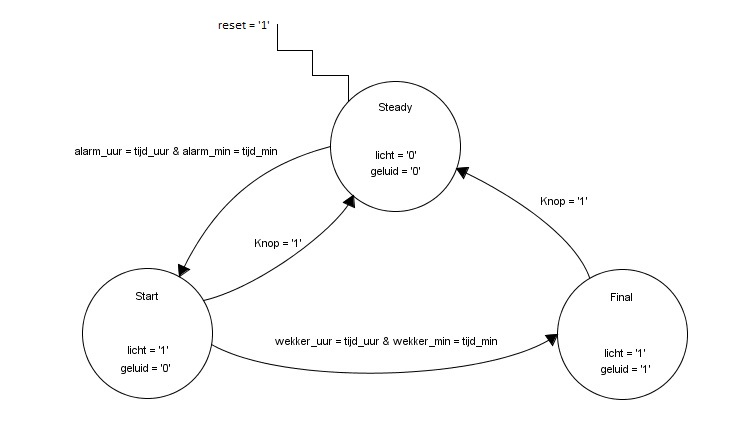
\includegraphics[width=\textwidth,height=\textheight,keepaspectratio]{FSM/alarm-compare-fsm.jpg}
FSM van ``alarm-counter", hier wordt de lengte van het PWM signaal berekend.

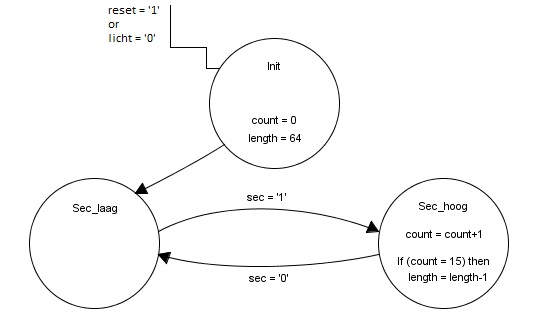
\includegraphics[width=\textwidth,height=\textheight,keepaspectratio]{FSM/alarm-count-fsm.jpg}
\newpage
FSM van ``alarm-pwm", hier wordt het pwm signaal gegenereed wat de led aanstuurt.

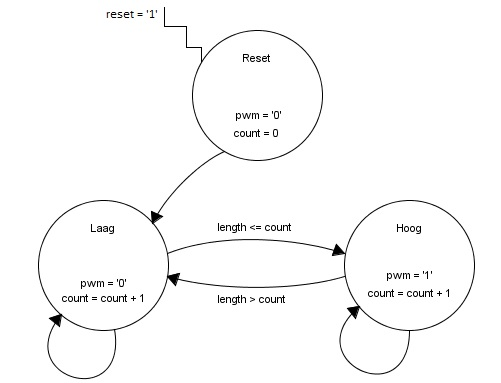
\includegraphics[width=\textwidth,height=\textheight,keepaspectratio]{FSM/alarm-pwm-fsm.jpg}
\subsection{Code}
De code voor het alarm is opgedeeld in 3 stukken:
\begin{itemize}[nolistsep]
\item alarm-compare
\item alarm-counter
\item alarm-pwm
\end{itemize}
Alarm-counter en alarm-pwm zijn onderdeel van een top entity, alarm. Omdat het nog niet zeker is waar alarm-compare geplaatst gaat worden op de chip is die daar niet bij inbegrepen.
De code voor het alarm is te vinden in \cref{Ap:code_alarm}.
\begin{itemize}[nolistsep]
\item De entity en behavioural van alarm compare is te vinden in \cref{code:ent_alarm_compare,code:beh_alarm_compare}.
\item De top entity en port map van alarm is te vinden in \cref{code:ent_alarm,code:beh_alarm}.
\item De entity en behavioural van alarm-counter is te vinden in \cref{code:ent_alarm_counter,code:beh_alarm_counter}.
\item De entity en behavioural van alarm-pwm is te vinden in \cref{code:ent_alarm_pwm,code:beh_alarm_pwm}.
\end{itemize}
\section{Resultaten}
Alle onderdelen werken in de simulaties. Zowel de simulatie van de behaviour als van de extracted vhdl.
Onderstaande afbeeldingen zijn de resultaten van de simulaties, eerst die van de behaviour daarna van de extracted.
De eerste 2 afbeedingen zijn van ``alarm-compare", de andere 2 van ``alarm-pwm".
\\

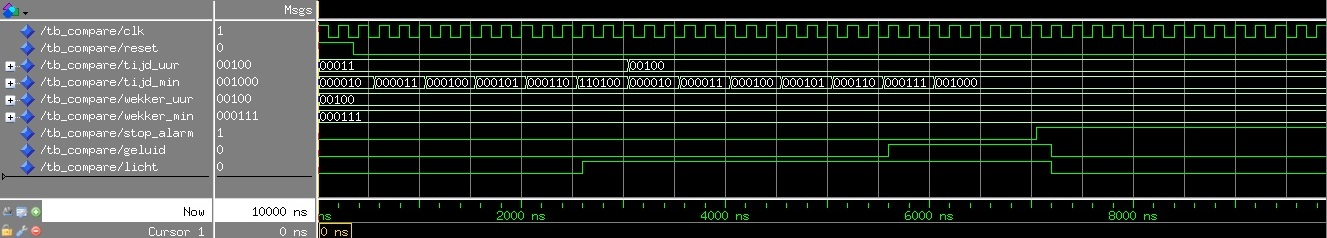
\includegraphics[width=\textwidth,height=\textheight,keepaspectratio]{results/compare.jpg}

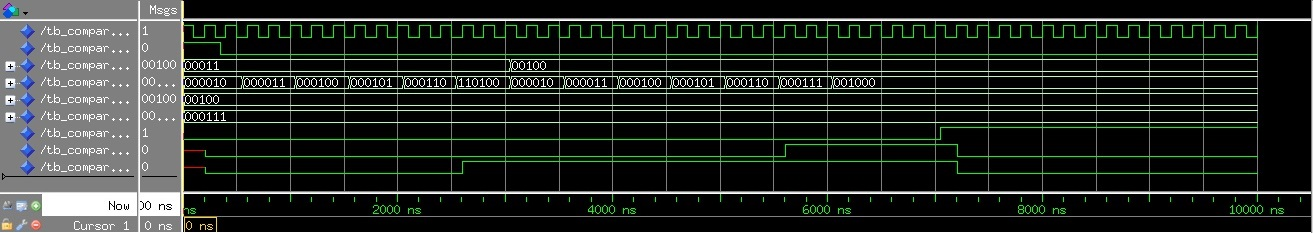
\includegraphics[width=\textwidth,height=\textheight,keepaspectratio]{results/compare_ext.jpg}
\\
\\
Te zien is in de 2 afbeeldingen hier boven dat wanneer de huidige tijd (tijd\_uur en tijd\_min) gelijk is aan de wekker tijd (wekker\_uur en wekker\_min) minus 15 minuten, dan gaat het signaal licht naar '1'. Als de huidige tijd gelijk is aan de wekker tijd, gaat ook het geluid signaal naar '1'.
Ook is te zien dat wanneer de knop (in de simulatie stop\_alarm) naar '1' gaat het licht en/of geluid weer naar '0' gaat.
\\

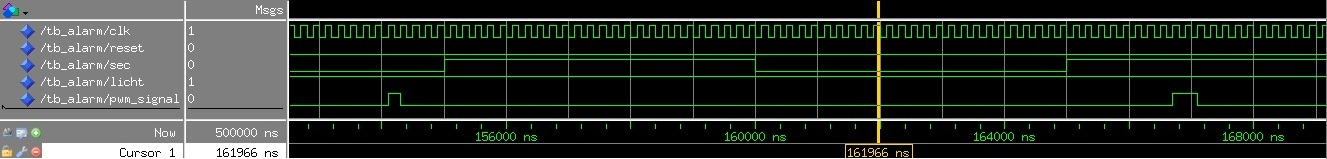
\includegraphics[width=\textwidth,height=\textheight,keepaspectratio]{results/alarm.jpg}
\\

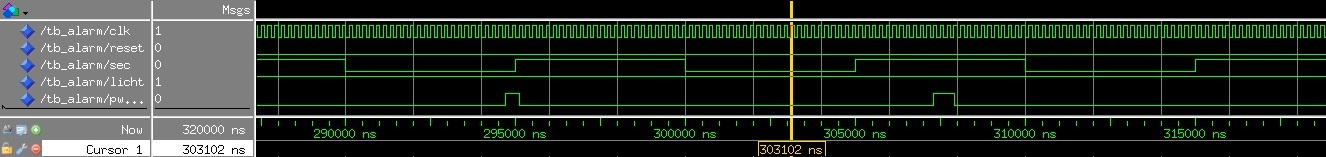
\includegraphics[width=\textwidth,height=\textheight,keepaspectratio]{results/alarm_ext.jpg}
\\
\\
Bovenstaande 2 afbeeldingen laten zien dat op het moment dat er 15 seconde zijn verstreken het pwm-signaal breder wordt.
